\documentclass[]{article}
\usepackage{lmodern}
\usepackage{amssymb,amsmath}
\usepackage{ifxetex,ifluatex}
\usepackage{fixltx2e} % provides \textsubscript
\ifnum 0\ifxetex 1\fi\ifluatex 1\fi=0 % if pdftex
  \usepackage[T1]{fontenc}
  \usepackage[utf8]{inputenc}
\else % if luatex or xelatex
  \ifxetex
    \usepackage{mathspec}
  \else
    \usepackage{fontspec}
  \fi
  \defaultfontfeatures{Ligatures=TeX,Scale=MatchLowercase}
\fi
% use upquote if available, for straight quotes in verbatim environments
\IfFileExists{upquote.sty}{\usepackage{upquote}}{}
% use microtype if available
\IfFileExists{microtype.sty}{%
\usepackage{microtype}
\UseMicrotypeSet[protrusion]{basicmath} % disable protrusion for tt fonts
}{}
\usepackage[margin=1in]{geometry}
\usepackage{hyperref}
\hypersetup{unicode=true,
            pdftitle={Atlas-PS 6},
            pdfauthor={David Atlas},
            pdfborder={0 0 0},
            breaklinks=true}
\urlstyle{same}  % don't use monospace font for urls
\usepackage{color}
\usepackage{fancyvrb}
\newcommand{\VerbBar}{|}
\newcommand{\VERB}{\Verb[commandchars=\\\{\}]}
\DefineVerbatimEnvironment{Highlighting}{Verbatim}{commandchars=\\\{\}}
% Add ',fontsize=\small' for more characters per line
\usepackage{framed}
\definecolor{shadecolor}{RGB}{248,248,248}
\newenvironment{Shaded}{\begin{snugshade}}{\end{snugshade}}
\newcommand{\KeywordTok}[1]{\textcolor[rgb]{0.13,0.29,0.53}{\textbf{{#1}}}}
\newcommand{\DataTypeTok}[1]{\textcolor[rgb]{0.13,0.29,0.53}{{#1}}}
\newcommand{\DecValTok}[1]{\textcolor[rgb]{0.00,0.00,0.81}{{#1}}}
\newcommand{\BaseNTok}[1]{\textcolor[rgb]{0.00,0.00,0.81}{{#1}}}
\newcommand{\FloatTok}[1]{\textcolor[rgb]{0.00,0.00,0.81}{{#1}}}
\newcommand{\ConstantTok}[1]{\textcolor[rgb]{0.00,0.00,0.00}{{#1}}}
\newcommand{\CharTok}[1]{\textcolor[rgb]{0.31,0.60,0.02}{{#1}}}
\newcommand{\SpecialCharTok}[1]{\textcolor[rgb]{0.00,0.00,0.00}{{#1}}}
\newcommand{\StringTok}[1]{\textcolor[rgb]{0.31,0.60,0.02}{{#1}}}
\newcommand{\VerbatimStringTok}[1]{\textcolor[rgb]{0.31,0.60,0.02}{{#1}}}
\newcommand{\SpecialStringTok}[1]{\textcolor[rgb]{0.31,0.60,0.02}{{#1}}}
\newcommand{\ImportTok}[1]{{#1}}
\newcommand{\CommentTok}[1]{\textcolor[rgb]{0.56,0.35,0.01}{\textit{{#1}}}}
\newcommand{\DocumentationTok}[1]{\textcolor[rgb]{0.56,0.35,0.01}{\textbf{\textit{{#1}}}}}
\newcommand{\AnnotationTok}[1]{\textcolor[rgb]{0.56,0.35,0.01}{\textbf{\textit{{#1}}}}}
\newcommand{\CommentVarTok}[1]{\textcolor[rgb]{0.56,0.35,0.01}{\textbf{\textit{{#1}}}}}
\newcommand{\OtherTok}[1]{\textcolor[rgb]{0.56,0.35,0.01}{{#1}}}
\newcommand{\FunctionTok}[1]{\textcolor[rgb]{0.00,0.00,0.00}{{#1}}}
\newcommand{\VariableTok}[1]{\textcolor[rgb]{0.00,0.00,0.00}{{#1}}}
\newcommand{\ControlFlowTok}[1]{\textcolor[rgb]{0.13,0.29,0.53}{\textbf{{#1}}}}
\newcommand{\OperatorTok}[1]{\textcolor[rgb]{0.81,0.36,0.00}{\textbf{{#1}}}}
\newcommand{\BuiltInTok}[1]{{#1}}
\newcommand{\ExtensionTok}[1]{{#1}}
\newcommand{\PreprocessorTok}[1]{\textcolor[rgb]{0.56,0.35,0.01}{\textit{{#1}}}}
\newcommand{\AttributeTok}[1]{\textcolor[rgb]{0.77,0.63,0.00}{{#1}}}
\newcommand{\RegionMarkerTok}[1]{{#1}}
\newcommand{\InformationTok}[1]{\textcolor[rgb]{0.56,0.35,0.01}{\textbf{\textit{{#1}}}}}
\newcommand{\WarningTok}[1]{\textcolor[rgb]{0.56,0.35,0.01}{\textbf{\textit{{#1}}}}}
\newcommand{\AlertTok}[1]{\textcolor[rgb]{0.94,0.16,0.16}{{#1}}}
\newcommand{\ErrorTok}[1]{\textcolor[rgb]{0.64,0.00,0.00}{\textbf{{#1}}}}
\newcommand{\NormalTok}[1]{{#1}}
\usepackage{longtable,booktabs}
\usepackage{graphicx,grffile}
\makeatletter
\def\maxwidth{\ifdim\Gin@nat@width>\linewidth\linewidth\else\Gin@nat@width\fi}
\def\maxheight{\ifdim\Gin@nat@height>\textheight\textheight\else\Gin@nat@height\fi}
\makeatother
% Scale images if necessary, so that they will not overflow the page
% margins by default, and it is still possible to overwrite the defaults
% using explicit options in \includegraphics[width, height, ...]{}
\setkeys{Gin}{width=\maxwidth,height=\maxheight,keepaspectratio}
\IfFileExists{parskip.sty}{%
\usepackage{parskip}
}{% else
\setlength{\parindent}{0pt}
\setlength{\parskip}{6pt plus 2pt minus 1pt}
}
\setlength{\emergencystretch}{3em}  % prevent overfull lines
\providecommand{\tightlist}{%
  \setlength{\itemsep}{0pt}\setlength{\parskip}{0pt}}
\setcounter{secnumdepth}{0}
% Redefines (sub)paragraphs to behave more like sections
\ifx\paragraph\undefined\else
\let\oldparagraph\paragraph
\renewcommand{\paragraph}[1]{\oldparagraph{#1}\mbox{}}
\fi
\ifx\subparagraph\undefined\else
\let\oldsubparagraph\subparagraph
\renewcommand{\subparagraph}[1]{\oldsubparagraph{#1}\mbox{}}
\fi

%%% Use protect on footnotes to avoid problems with footnotes in titles
\let\rmarkdownfootnote\footnote%
\def\footnote{\protect\rmarkdownfootnote}

%%% Change title format to be more compact
\usepackage{titling}

% Create subtitle command for use in maketitle
\newcommand{\subtitle}[1]{
  \posttitle{
    \begin{center}\large#1\end{center}
    }
}

\setlength{\droptitle}{-2em}
  \title{Atlas-PS 6}
  \pretitle{\vspace{\droptitle}\centering\huge}
  \posttitle{\par}
  \author{David Atlas}
  \preauthor{\centering\large\emph}
  \postauthor{\par}
  \predate{\centering\large\emph}
  \postdate{\par}
  \date{10/2/2018}


\begin{document}
\maketitle

\newcommand{\Z}[1]{\left(\frac{x_{#1} - \mu_{#1}}{\sigma_{#1}} \right)}






\section{Problem 1}\label{problem-1}

\subsection{a)}\label{a}

To show that the Metropolis-Hastings ratio will always be equal to 1
when \(g(\cdot \vert x^{(t)}) = f(\cdot \vert x^{(t)})\), we first
define the ratio \[
R(x^{(t)}, X^*)=\frac{f(X^*) g(x^{(t)} \vert X^*)}{f(x^{(t)}) g(X^*|x^{(t)})}.
\]

Note that
\(g(\cdot \vert x^{(t)}) = f(\cdot \vert x^{(t)}) \forall x^{(t)} \implies f(X^*|x^{(t)}) = g(X^*|x^{(t)})\)
and \$ f(X\^{}\{(t)\} \textbar{} X\^{}\emph{) = g(X\^{}\{(t)\}
\textbar{} X\^{}})\$. In the Metropolis-Hastings Ratio, \(f\) is not
conditional on previous values of the simulation, as it is the target
distribution that we want to converge on. Therefore,
\(f(X^*) = g(X^*|x^{(t)})\) and
\(f(X^{(t)}) = g(X^{(t)} | X^*) \forall x^{(t)}\).

Now, it is trivial to show that \[
R(x^{(t)}, X^*)=\frac{g(x^{(t)} \vert X^*) f(X^*) }{f(x^{(t)}) g(X^*|x^{(t)})} = \frac{f(x^{(t)} \vert X^*) f(X^*) }{f(x^{(t)}) f(X^*|x^{(t)})} =  \frac{f(x^{(t)}) f(X^*) }{f(x^{(t)}) f(X^*)} = 1.
\]

This is intuitive too, as if the proposal distribution is equal to the
target distribution, any draw from the proposal distribution should be
included in the chain, and this will lead to convergence on the target
distribution.

\subsection{b)}\label{b}

We start with the definition of the conditional distribution \[
f_{X_1 | X_2}(x_1 | x_2) = \frac{f(x_1, x_2)}{f_{X_2}(x_2)},
\] or that the conditional distribution is equal to the joint
distribution divided by the marginal distribution of the conditioning
variable.

This implies that \[
\frac{f_{X_1|X_2}(x_1|x_2)}{f_{X_2|X_1}(x_2|x_1)} = \frac{f(x_1, x_2)f_{X_1}(x_1)}{f_{X_2}(x_2)f(x_1, x_2)} = \frac{f_{X_1}(x_1)}{f_{X_2}(x_2)}.
\]

Integrating both sides of the equation with respect to \(dx_1\), we get
\[
\int_{-\infty}^{\infty}\frac{f_{X_1|X_2}(x_1|x_2)}{f_{X_2|X_1}(x_2|x_1)} dx_1 = \int_{-\infty}^{\infty} \frac{f_{X_1}(x_1)}{f_{X_2}(x_2)}dx_1 = \frac{1}{f_{X_2}(x_2)}
\] because \(\int_{-\infty}^{\infty} f_{X_1}(x_1)dx_1 = 1\), as
\(f_{X_1}\) is a probability distribution.

We reference the equations above to show that \[
f_{X_2}(x_2) = \frac{f(x_1, x_2)}{f_{X_1 | X_2}(x_1 | x_2)}
\] implying \[
\frac{1}{\int_{-\infty}^{\infty}\frac{f_{X_1|X_2}(x_1|x_2)}{f_{X_2|X_1}(x_2|x_1)} dx_1} = 
f_{X_2}(x_2) = \frac{f(x_1, x_2)}{f_{X_1 | X_2}(x_1 | x_2)}.
\]

Multiplying across, we can say that \[
f(x_1, x_2) = \frac{f_{X_1 | X_2}(x_1 | x_2)}{\int_{-\infty}^{\infty}\frac{f_{X_1|X_2}(x_1|x_2)}{f_{X_2|X_1}(x_2|x_1)} dx_1}.
\]

\section{Problem 2}\label{problem-2}

\subsection{a)}\label{a-1}

We begin with the bivariate normal distribution: \[
f_{X_1X_2}(x_1, x_2) = \frac{1}{2 \pi \sigma_1 \sigma_2 \sqrt{1 - \rho^2}} 
\rm{e}^{-\frac{1}{2(1 - \rho^2)}\left[\left(\frac{x_1 - \mu_1}{\sigma_1}\right)^2 -2 \rho \left(\frac{x_1-\mu_1}{\sigma_1} \right) 
\left(\frac{x_2 - \mu_2}{\sigma_2}\right) + \left(\frac{x_2-\mu_2}{\sigma_2}\right)^2.
\right]}
\]

We note that the conditional density
\(f_{X_1|X_2}(x_1 | x_2) = \frac{f_{X_1 X_2}(x_1, x_2)}{f_{X_2}(x_2)}\).
In this case, this means that \[
f_{X_1|X_2}(x_1 | x_2) =
\frac{\frac{1}{2 \pi \sigma_1 \sigma_2 \sqrt{1 - \rho^2}} 
\rm{e}^{-\frac{1}{2}\left[\left(\frac{x_1 - \mu_1}{\sigma_1}\right)^2 -2 \rho \left(\frac{x_1-\mu_1}{\sigma_1} \right) 
\left(\frac{x_2 - \mu_2}{\sigma_2}\right) + \left(\frac{x_2-\mu_2}{\sigma_2}\right)^2.
\right]}}
{\frac{1}{\sqrt{2\pi\sigma_2^2}} \rm{e}^{-\frac{1}{2}\left(\frac{x_2 - \mu_2}{\sigma_2}^2 \right)}}
\]

We can rewrite the exponent of the exponential of the bivariate normal
as follows: \[
-\frac{1}{2(1-\rho^2)}\Z{1}^2 - 2 \rho\Z{1}\Z{2} + \rho^2\Z{2}^2 + (1 - \rho^2)\Z{2}^2.
\]

Therefore, expanding our terms and cancelling out where possible, we can
write the conditional density as \[
f_{X_1|X_2}(x_1 | x_2) = \frac{1}{\sqrt{2\pi\sigma_1^2(1-\rho^2)}} \rm{e}^
{-\frac{1}{2(1-\rho^2)}\left[
\Z{1}^2 - 2 \rho \Z{1}\Z{2} + \rho^2 \Z{2}^2
\right] }
\]

Note that the above exponent of the exponential function can be
rewritten:

\begin{align*}
\Z{1}^2 - 2 \rho \Z{1}\Z{2} + \rho^2 \Z{2}^2 &= 
\left(
\Z{1} - \rho\Z{2}^2
\right)^2 \\ 
&= \frac{1}{\sigma_1^2}\left((x_1 - \mu_1) - \rho \frac{\sigma_1}{\sigma_2}(x_2 - \mu_2)\right)^2
\end{align*}

such that the conditional probability can be written as \[
f_{X_1|X_2}(x_1 | x_2) = 
\frac{1}{\sqrt{2\pi\sigma_1^2(1-\rho^2)}} \rm{e}^{
-\frac{1}{2}
\frac{\left(x_1 - \mu_1 - \rho \frac{\sigma_1}{\sigma_2}(x_2 - \mu_2)\right)^2}{\sigma_1^2(1-\rho^2)}
}.
\]

Given the symmetric nature of the density, we can write \[
f_{X_2|X_1}(x_2 | x_1)=
\frac{1}{\sqrt{2\pi\sigma_2^2(1-\rho^2)}} \rm{e}^{
-\frac{1}{2}
\frac{\left(x_2 - \mu_2 - \rho \frac{\sigma_2}{\sigma_1}(x_1 - \mu_1)\right)^2}{\sigma_2^2(1-\rho^2)}
}
\]

Note that these are both normally distributed variables, so we can write
that

\begin{align*}
X_1 | X_2 &\sim N(\mu_1 + \rho \frac{\sigma_2}{\sigma_1}(x_2 - \mu_2), \sigma_1^2(1 - \rho^2)) \\
X_2 | X_1 &\sim N(\mu_2 + \rho \frac{\sigma_1}{\sigma_2}(x_1 - \mu_1), \sigma_2^2(1 - \rho^2))
\end{align*}

\subsection{b)}\label{b-1}

Next, we generate Gibbs samples to determine if these distributions can
be simulated with that methodology. We assume the variables are standard
normal, with varying correlations.

\begin{Shaded}
\begin{Highlighting}[]
\CommentTok{# Define the conditional distributions}
\NormalTok{one_given_two <-}\StringTok{ }\NormalTok{function(rho, x2) }\KeywordTok{rnorm}\NormalTok{(}\DataTypeTok{n=}\DecValTok{1}\NormalTok{, }\DataTypeTok{mean=}\NormalTok{(rho *}\StringTok{ }\NormalTok{x2), }\DataTypeTok{sd=}\NormalTok{(}\DecValTok{1}\NormalTok{-rho^}\DecValTok{2}\NormalTok{))}
\NormalTok{two_given_one <-}\StringTok{ }\NormalTok{function(rho, x1) }\KeywordTok{rnorm}\NormalTok{(}\DataTypeTok{n=}\DecValTok{1}\NormalTok{, }\DataTypeTok{mean=}\NormalTok{(rho *}\StringTok{ }\NormalTok{x1), }\DataTypeTok{sd=}\NormalTok{(}\DecValTok{1}\NormalTok{-rho^}\DecValTok{2}\NormalTok{))}

\CommentTok{# Generate 1000 samples from each}
\NormalTok{data_list <-}\StringTok{ }\KeywordTok{lapply}\NormalTok{(}\KeywordTok{seq}\NormalTok{(}\DecValTok{0}\NormalTok{, .}\DecValTok{5}\NormalTok{, .}\DecValTok{1}\NormalTok{), function(rho)\{}
  \NormalTok{x2 <-}\StringTok{ }\DecValTok{0}
  \NormalTok{samples <-}\StringTok{ }\KeywordTok{matrix}\NormalTok{(}\DataTypeTok{ncol=}\DecValTok{2}\NormalTok{, }\DataTypeTok{nrow=}\DecValTok{0}\NormalTok{)}
  \NormalTok{for(i in }\DecValTok{1}\NormalTok{:}\DecValTok{5000}\NormalTok{)\{}
    \CommentTok{# Get the samples}
    \NormalTok{x1 <-}\StringTok{ }\KeywordTok{one_given_two}\NormalTok{(rho, x2)}
    \NormalTok{x2 <-}\StringTok{ }\KeywordTok{two_given_one}\NormalTok{(rho, x1)}
    \NormalTok{samples <-}\StringTok{ }\KeywordTok{rbind}\NormalTok{(samples, }\KeywordTok{c}\NormalTok{(x1, x2))}
  \NormalTok{\}}
  \KeywordTok{return}\NormalTok{(samples)}
\NormalTok{\})}
\end{Highlighting}
\end{Shaded}

To determine whether or not Gibbs sampling is a viable method here, we
check the estimated parameters against their true values. We note that
the mean is well estimated in all the samples, so we'll examine only the
covariance matrix for each of the iterations.

\begin{Shaded}
\begin{Highlighting}[]
\NormalTok{estimates <-}\StringTok{ }\KeywordTok{lapply}\NormalTok{(}\KeywordTok{seq}\NormalTok{(}\DecValTok{1}\NormalTok{, }\KeywordTok{length}\NormalTok{(data_list)), function(i)\{}
  \NormalTok{data_ <-}\StringTok{ }\NormalTok{data_list[[i]]}
  \NormalTok{rho <-}\StringTok{ }\KeywordTok{seq}\NormalTok{(}\DecValTok{0}\NormalTok{, .}\DecValTok{5}\NormalTok{, .}\DecValTok{1}\NormalTok{)[i]}
  \NormalTok{res <-}\StringTok{ }\KeywordTok{lapply}\NormalTok{(}\KeywordTok{seq}\NormalTok{(}\DecValTok{1000}\NormalTok{, }\KeywordTok{nrow}\NormalTok{(data_) -}\StringTok{ }\DecValTok{1}\NormalTok{, }\DecValTok{1000}\NormalTok{), function(burnin)\{}
    \CommentTok{# Get the burnin data only}
    \NormalTok{data <-}\StringTok{ }\NormalTok{data_[burnin:}\KeywordTok{nrow}\NormalTok{(data_), ]}
    \CommentTok{# Get the covariance matrix}
    \KeywordTok{data.frame}\NormalTok{(}\KeywordTok{cov}\NormalTok{(data))}
  \NormalTok{\})}
  \NormalTok{res}
\NormalTok{\})}
\end{Highlighting}
\end{Shaded}

(Note: Not printing the results here because it was many dataframes, but
I took a look at the output manually.)

Inspecting the results, we see that the correlation between the two
variables creates a problem. All of the parameters are estimates well,
except the variances of the individual variables. Because the variables
are correlated, they clearly have a tendency to exhibit smaller
variances together.

When there is no correlation, the sampling works well. As the
correlation grows, the parameter estimates for the variance and the
correlation degrades. Gibbs Sampling may not work so well for estimating
all of the parameters here.

\section{Problem 3}\label{problem-3}

\subsection{a) MCdata1.txt}\label{a-mcdata1.txt}

We read in the first dataset from Blackboard.

\begin{Shaded}
\begin{Highlighting}[]
\NormalTok{mc_data1 <-}\StringTok{ }\KeywordTok{scan}\NormalTok{(}\StringTok{"Module 6 Data Sets/MCdata1.txt"}\NormalTok{)}
\end{Highlighting}
\end{Shaded}

We plot the sample path for the first MC.

\begin{Shaded}
\begin{Highlighting}[]
\KeywordTok{plot}\NormalTok{(mc_data1, }\DataTypeTok{type =}  \StringTok{'l'}\NormalTok{, }\DataTypeTok{main=}\StringTok{'MCData1.txt'}\NormalTok{, }\DataTypeTok{ylab=}\StringTok{'X'}\NormalTok{)}
\end{Highlighting}
\end{Shaded}

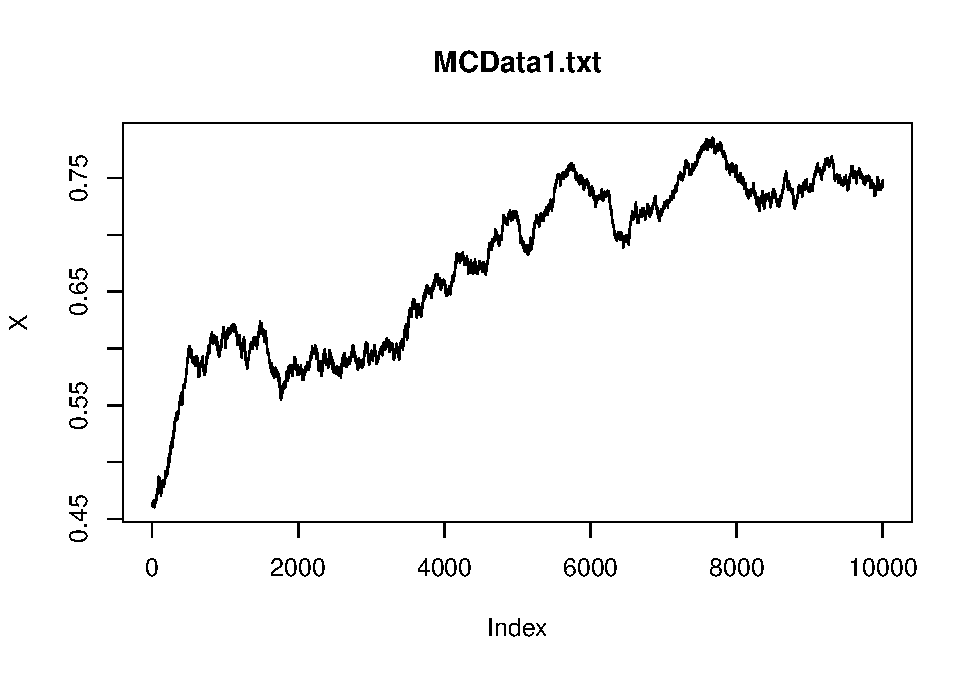
\includegraphics{Atlas-PS_6_files/figure-latex/unnamed-chunk-4-1.pdf} We
plot the CUMSUM diagnostic plot next.

\begin{Shaded}
\begin{Highlighting}[]
\NormalTok{mu <-}\StringTok{ }\KeywordTok{mean}\NormalTok{(mc_data1)}
\KeywordTok{plot}\NormalTok{(}\KeywordTok{cumsum}\NormalTok{(mc_data1 -}\StringTok{ }\NormalTok{mu), }\DataTypeTok{type=}\StringTok{'l'}\NormalTok{, }\DataTypeTok{main=}\StringTok{'CUMSUM Plot'}\NormalTok{, }\DataTypeTok{ylab=}\StringTok{''}\NormalTok{)}
\end{Highlighting}
\end{Shaded}

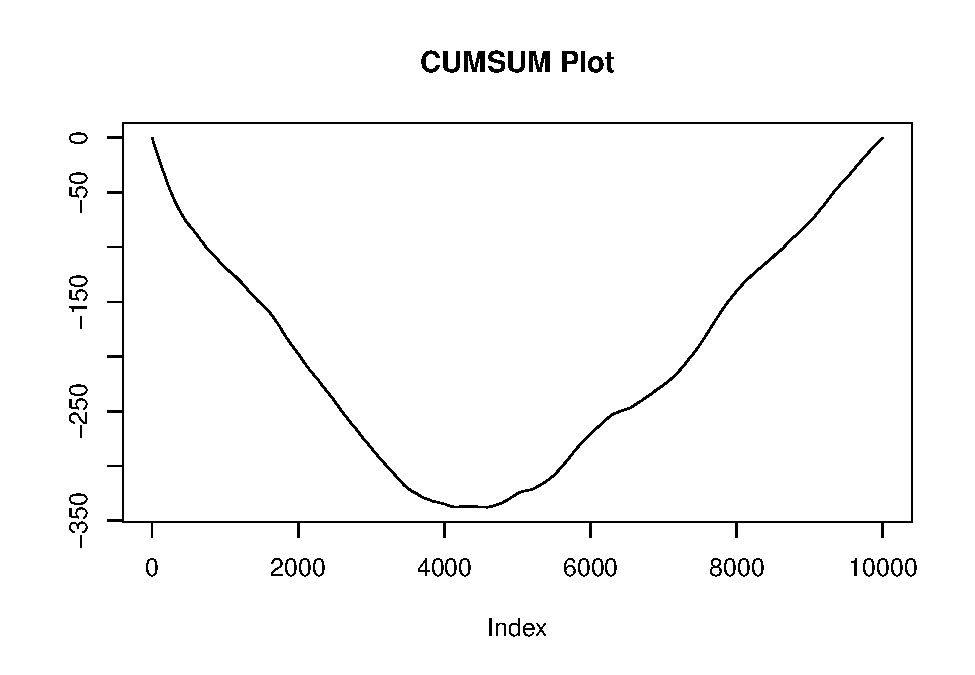
\includegraphics{Atlas-PS_6_files/figure-latex/unnamed-chunk-5-1.pdf}

Next, we plot the autocorrelation plot for the chain.

\begin{Shaded}
\begin{Highlighting}[]
\NormalTok{autocorr <-}\StringTok{ }\NormalTok{function(data, lag)\{}
  \NormalTok{ct <-}\StringTok{ }\KeywordTok{cov}\NormalTok{(data[}\DecValTok{1}\NormalTok{:}\StringTok{ }\NormalTok{(}\KeywordTok{length}\NormalTok{(data) -}\StringTok{ }\NormalTok{lag +}\StringTok{ }\DecValTok{1}\NormalTok{)], data[lag :}\KeywordTok{length}\NormalTok{(data)])}
  \NormalTok{c0 <-}\StringTok{ }\KeywordTok{var}\NormalTok{(data[}\DecValTok{1}\NormalTok{:}\StringTok{ }\NormalTok{(}\KeywordTok{length}\NormalTok{(data) -}\StringTok{ }\NormalTok{lag +}\StringTok{ }\DecValTok{1}\NormalTok{)])}
  \KeywordTok{return}\NormalTok{(ct /}\StringTok{ }\NormalTok{c0)}
\NormalTok{\}  }
\NormalTok{n <-}\StringTok{ }\DecValTok{2000}
\KeywordTok{plot}\NormalTok{(}\KeywordTok{seq}\NormalTok{(}\DecValTok{2}\NormalTok{, n, }\DecValTok{20}\NormalTok{), }\KeywordTok{sapply}\NormalTok{(}\KeywordTok{seq}\NormalTok{(}\DecValTok{2}\NormalTok{, n, }\DecValTok{20}\NormalTok{), function(lag) }\KeywordTok{autocorr}\NormalTok{(mc_data1, lag)), }
     \DataTypeTok{type=}\StringTok{'h'}\NormalTok{, }\DataTypeTok{ylim=}\KeywordTok{c}\NormalTok{(-.}\DecValTok{2}\NormalTok{, }\DecValTok{1}\NormalTok{), }\DataTypeTok{xlab=}\StringTok{"Lag"}\NormalTok{, }\DataTypeTok{ylab=}\StringTok{"Autocorrelation"}\NormalTok{)}
\end{Highlighting}
\end{Shaded}

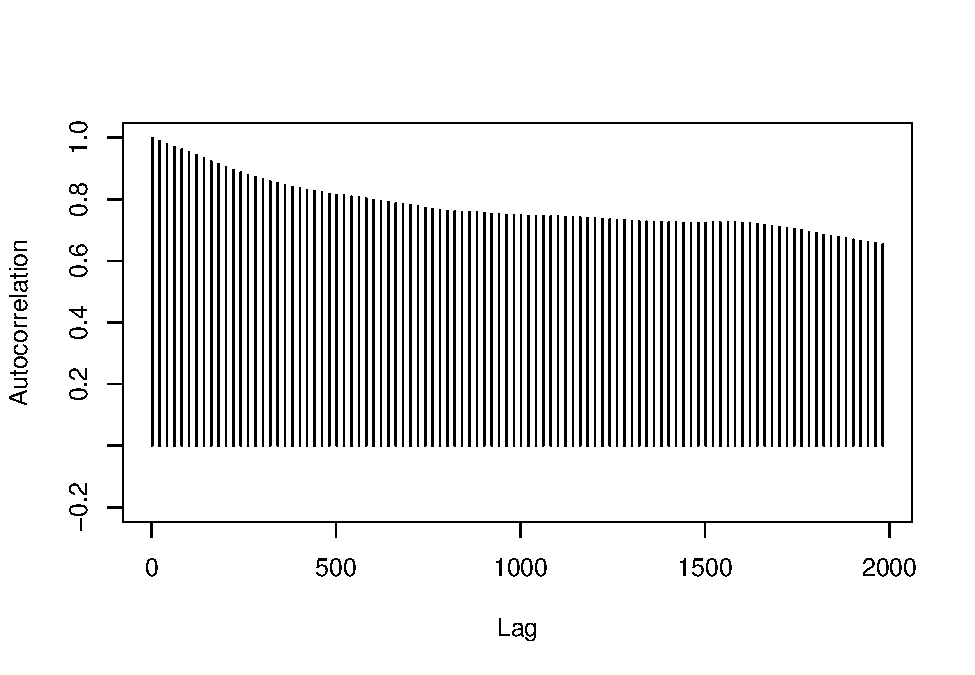
\includegraphics{Atlas-PS_6_files/figure-latex/unnamed-chunk-6-1.pdf}

Combining all three of the diagnostic plots, it seems as though the
chain is not mixing well. The first plot shows the chain getting stuck
in varies regions, but not bouncing around a specified region (the range
of the stationary distribution).

The second plot does not show a CUMSUM that is wiggly with small
excursions from zero. It's pretty clear that even if we included a
burnin period, this would still be the case.

The third plot shows that the autocorrelation decays extremely slowly.
Above, we show 2000 lags, and the autocorrelation is pretty strong
throughout.

It seems as though this chain isn't mixing well, and is not converging
at all.

\subsection{b) MCdata2.txt}\label{b-mcdata2.txt}

We read in the second dataset from Blackboard.

\begin{Shaded}
\begin{Highlighting}[]
\NormalTok{mc_data2 <-}\StringTok{ }\KeywordTok{scan}\NormalTok{(}\StringTok{"Module 6 Data Sets/MCdata2.txt"}\NormalTok{)}
\end{Highlighting}
\end{Shaded}

We plot the sample path for the first MC.

\begin{Shaded}
\begin{Highlighting}[]
\KeywordTok{plot}\NormalTok{(mc_data2, }\DataTypeTok{type =}  \StringTok{'l'}\NormalTok{, }\DataTypeTok{main=}\StringTok{'MCData2.txt'}\NormalTok{, }\DataTypeTok{ylab=}\StringTok{'X'}\NormalTok{)}
\end{Highlighting}
\end{Shaded}

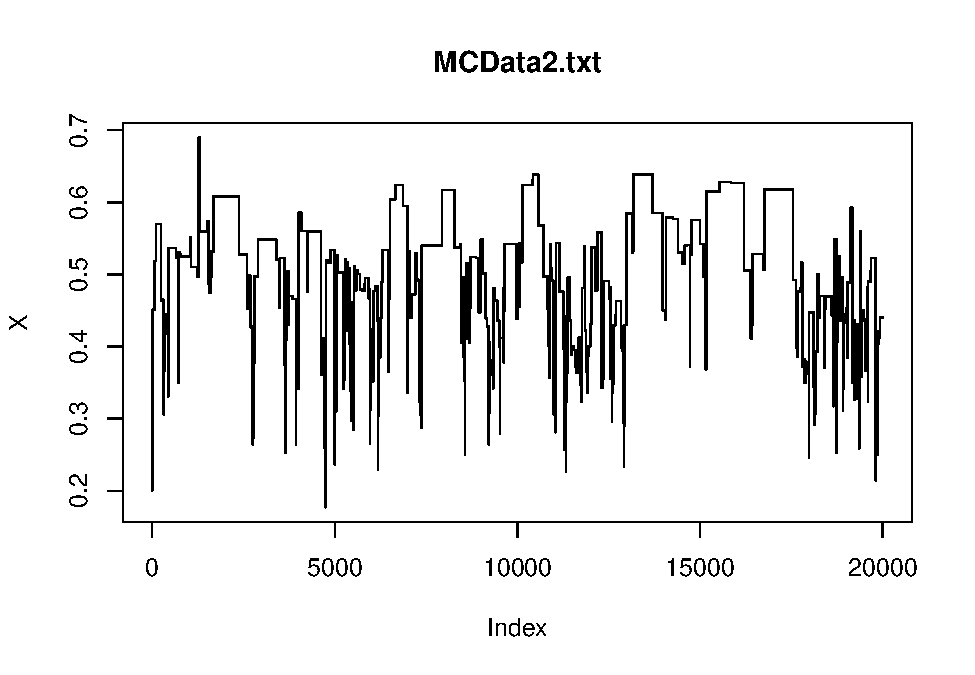
\includegraphics{Atlas-PS_6_files/figure-latex/unnamed-chunk-8-1.pdf} We
plot the CUMSUM diagnostic plot next.

\begin{Shaded}
\begin{Highlighting}[]
\NormalTok{mu <-}\StringTok{ }\KeywordTok{mean}\NormalTok{(mc_data2)}
\KeywordTok{plot}\NormalTok{(}\KeywordTok{cumsum}\NormalTok{(mc_data2 -}\StringTok{ }\NormalTok{mu), }\DataTypeTok{type=}\StringTok{'l'}\NormalTok{, }\DataTypeTok{main=}\StringTok{'CUMSUM Plot'}\NormalTok{, }\DataTypeTok{ylab=}\StringTok{''}\NormalTok{)}
\end{Highlighting}
\end{Shaded}

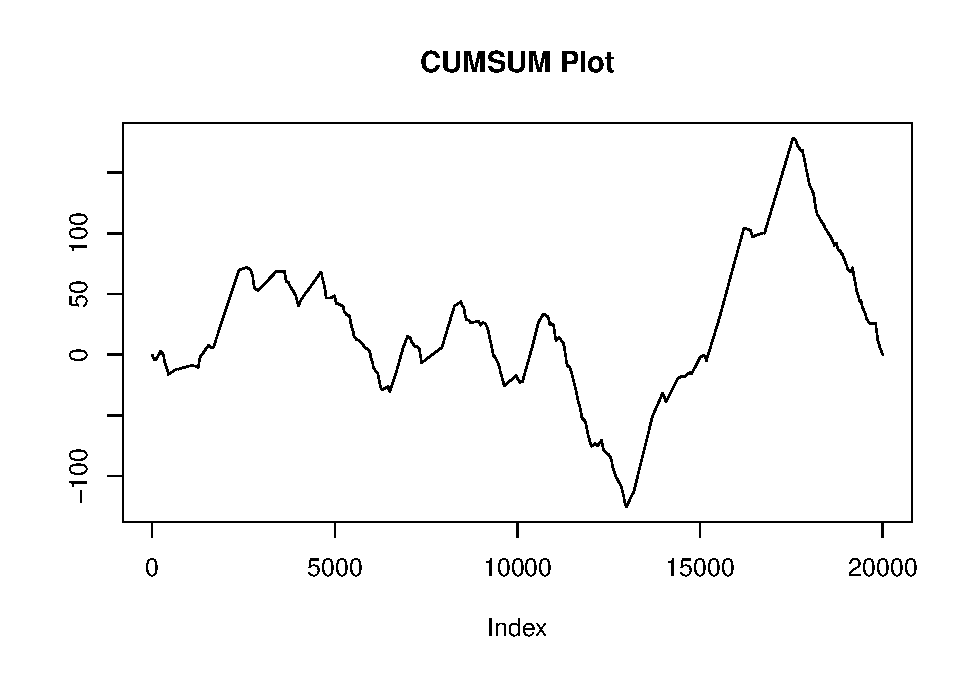
\includegraphics{Atlas-PS_6_files/figure-latex/unnamed-chunk-9-1.pdf}

Next, we plot the autocorrelation plot for the chain.

\begin{Shaded}
\begin{Highlighting}[]
\NormalTok{n <-}\StringTok{ }\DecValTok{40}
\KeywordTok{plot}\NormalTok{(}\KeywordTok{seq}\NormalTok{(}\DecValTok{2}\NormalTok{, n, }\DecValTok{1}\NormalTok{), }\KeywordTok{sapply}\NormalTok{(}\KeywordTok{seq}\NormalTok{(}\DecValTok{2}\NormalTok{, n, }\DecValTok{1}\NormalTok{), function(lag) }\KeywordTok{autocorr}\NormalTok{(mc_data2, lag)), }
     \DataTypeTok{type=}\StringTok{'h'}\NormalTok{, }\DataTypeTok{ylim=}\KeywordTok{c}\NormalTok{(-.}\DecValTok{2}\NormalTok{, }\DecValTok{1}\NormalTok{), }\DataTypeTok{xlab=}\StringTok{"Lag"}\NormalTok{, }\DataTypeTok{ylab=}\StringTok{"Autocorrelation"}\NormalTok{)}
\end{Highlighting}
\end{Shaded}

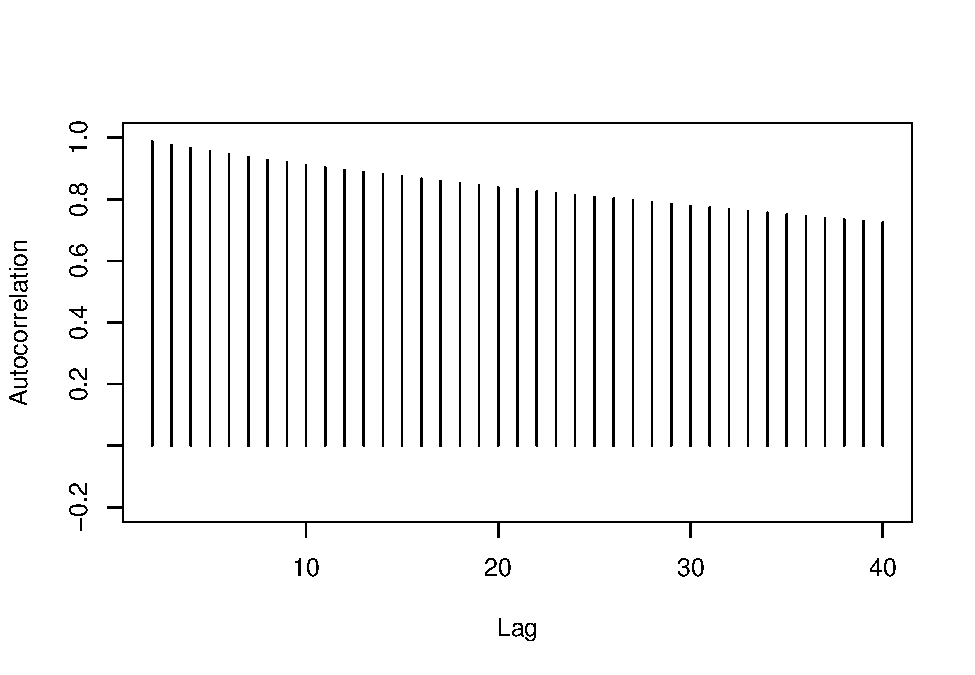
\includegraphics{Atlas-PS_6_files/figure-latex/unnamed-chunk-10-1.pdf}

Based on the three plots above, this chain appears to be somewhat mixing
effectively, although not at a rate that would be ideal.

The sample plot shows that the chain is yields points between .2 and .65
with varying frequencies. It seems to have periods of difficulty where
it gets stuck in ranges. But it doesn't stay that way for very long.

The CUMSUM plot sticks around zero, especially at first, but eventually
deviates far from there. It rebounds back towards zero, but only after a
while.

The autocorrelation plot shows decay, but not very quickly.

It seems as though, while the chain is mixing well, it hasn't converged
on the stationary distribution.

\section{Problem 5}\label{problem-5}

First, we read in the Markov Chain from the files.

\begin{Shaded}
\begin{Highlighting}[]
\NormalTok{chain_list <-}\StringTok{ }\KeywordTok{lapply}\NormalTok{(}\KeywordTok{seq}\NormalTok{(}\DecValTok{1}\NormalTok{, }\DecValTok{7}\NormalTok{), function(i) }\KeywordTok{scan}\NormalTok{(}\KeywordTok{paste0}\NormalTok{(}\StringTok{"Module 6 Data Sets/Chain "}\NormalTok{, i), }\DataTypeTok{skip=}\DecValTok{1}\NormalTok{))}
\end{Highlighting}
\end{Shaded}

Next, we define the needed expressions. It's all pretty simple algebra
straight out of the text.

\begin{Shaded}
\begin{Highlighting}[]
\NormalTok{cut_chain <-}\StringTok{ }\NormalTok{function(chain, D, L)\{}
  \KeywordTok{return}\NormalTok{(chain[D:}\StringTok{ }\NormalTok{(D +}\StringTok{ }\NormalTok{L)])}
\NormalTok{\}}

\NormalTok{get_xbar_j <-}\StringTok{ }\NormalTok{function(chain_list, D, L)\{}
  \KeywordTok{return}\NormalTok{(}\KeywordTok{sapply}\NormalTok{(chain_list, function(chain)\{}
    \KeywordTok{mean}\NormalTok{(}\KeywordTok{cut_chain}\NormalTok{(chain, D, L))}
  \NormalTok{\}))}
\NormalTok{\}}

\NormalTok{get_xbar <-}\StringTok{ }\NormalTok{function(chain_list, D, L)\{}
  \KeywordTok{return}\NormalTok{(}\KeywordTok{mean}\NormalTok{(}\KeywordTok{get_xbar_j}\NormalTok{(chain_list, D, L)))}
\NormalTok{\}}

\NormalTok{get_B <-}\StringTok{ }\NormalTok{function(data_list, D, L)\{}
  \NormalTok{J <-}\StringTok{ }\KeywordTok{length}\NormalTok{(data_list)}
  \KeywordTok{return}\NormalTok{((L /}\StringTok{ }\NormalTok{(J -}\StringTok{ }\DecValTok{1}\NormalTok{)) *}\StringTok{ }\KeywordTok{sum}\NormalTok{((}\KeywordTok{get_xbar_j}\NormalTok{(data_list, D, L) -}\StringTok{ }\KeywordTok{get_xbar}\NormalTok{(data_list, D, L)) ^}\StringTok{ }\DecValTok{2}\NormalTok{))}
\NormalTok{\}}

\NormalTok{get_s2_j <-}\StringTok{ }\NormalTok{function(chain_list, D, L)\{}
  \KeywordTok{sapply}\NormalTok{(chain_list, function(chain)\{}
    \NormalTok{chain_ <-}\StringTok{ }\KeywordTok{cut_chain}\NormalTok{(chain, D, L)}
    \NormalTok{xbarj <-}\StringTok{ }\KeywordTok{mean}\NormalTok{(chain_)}
    \KeywordTok{return}\NormalTok{((}\DecValTok{1} \NormalTok{/}\StringTok{ }\NormalTok{(L -}\StringTok{ }\DecValTok{1}\NormalTok{)) *}\StringTok{ }\KeywordTok{sum}\NormalTok{((chain_ -}\StringTok{ }\NormalTok{xbarj)^}\DecValTok{2}\NormalTok{))}
  \NormalTok{\})}
\NormalTok{\}}

\NormalTok{get_W <-}\StringTok{ }\NormalTok{function(data_list, D, L)\{}
  \KeywordTok{mean}\NormalTok{(}\KeywordTok{get_s2_j}\NormalTok{(data_list, D, L))}
\NormalTok{\}}

\NormalTok{get_R <-}\StringTok{ }\NormalTok{function(data_list, D, L)\{}
  \NormalTok{B <-}\StringTok{ }\KeywordTok{get_B}\NormalTok{(data_list, D, L)}
  \NormalTok{W <-}\StringTok{ }\KeywordTok{get_W}\NormalTok{(data_list, D, L)}
  \KeywordTok{return}\NormalTok{((((L -}\StringTok{ }\DecValTok{1}\NormalTok{) /}\StringTok{ }\NormalTok{L) *}\StringTok{ }\NormalTok{W +}\StringTok{ }\NormalTok{(}\DecValTok{1} \NormalTok{/}\StringTok{ }\NormalTok{L) *}\StringTok{ }\NormalTok{B) /}\StringTok{ }\NormalTok{W)}
\NormalTok{\}}
\end{Highlighting}
\end{Shaded}

Next, we run the code for each of the values of \(D\) and \(L\) in the
assignment.

\begin{Shaded}
\begin{Highlighting}[]
\NormalTok{D <-}\StringTok{ }\KeywordTok{c}\NormalTok{(}\DecValTok{0}\NormalTok{, }\DecValTok{500}\NormalTok{, }\DecValTok{0}\NormalTok{, }\DecValTok{250}\NormalTok{, }\DecValTok{0}\NormalTok{, }\DecValTok{25}\NormalTok{)}
\NormalTok{L <-}\StringTok{ }\KeywordTok{c}\NormalTok{(}\DecValTok{1000}\NormalTok{, }\DecValTok{500}\NormalTok{, }\DecValTok{500}\NormalTok{, }\DecValTok{250}\NormalTok{, }\DecValTok{50}\NormalTok{, }\DecValTok{25}\NormalTok{)}
\NormalTok{parameters <-}\StringTok{ }\KeywordTok{data.frame}\NormalTok{(}\DataTypeTok{D=}\NormalTok{D, }\DataTypeTok{L=}\NormalTok{L)}

\NormalTok{parameters$sqrt_R <-}\StringTok{ }\KeywordTok{sapply}\NormalTok{(}\KeywordTok{seq}\NormalTok{(}\DecValTok{1}\NormalTok{, }\KeywordTok{length}\NormalTok{(L)), function(i)\{}
  \KeywordTok{sqrt}\NormalTok{(}\KeywordTok{get_R}\NormalTok{(chain_list, }\DataTypeTok{D=}\NormalTok{parameters$D[i], parameters$L[i]))}
\NormalTok{\})}

\NormalTok{parameters$B <-}\StringTok{ }\KeywordTok{sapply}\NormalTok{(}\KeywordTok{seq}\NormalTok{(}\DecValTok{1}\NormalTok{, }\KeywordTok{length}\NormalTok{(L)), function(i)\{}
  \KeywordTok{get_B}\NormalTok{(chain_list, }\DataTypeTok{D=}\NormalTok{parameters$D[i], parameters$L[i])}
\NormalTok{\})}

\NormalTok{parameters$W <-}\StringTok{ }\KeywordTok{sapply}\NormalTok{(}\KeywordTok{seq}\NormalTok{(}\DecValTok{1}\NormalTok{, }\KeywordTok{length}\NormalTok{(L)), function(i)\{}
  \KeywordTok{get_W}\NormalTok{(chain_list, }\DataTypeTok{D=}\NormalTok{parameters$D[i], parameters$L[i])}
\NormalTok{\})}

\NormalTok{knitr::}\KeywordTok{kable}\NormalTok{(parameters, }\DataTypeTok{col.names =} \KeywordTok{c}\NormalTok{(}\StringTok{"D"}\NormalTok{, }\StringTok{"L"}\NormalTok{, }\StringTok{"sqrt(R)"}\NormalTok{, }\StringTok{"B"}\NormalTok{, }\StringTok{"W"}\NormalTok{))}
\end{Highlighting}
\end{Shaded}

\begin{longtable}[]{@{}rrrrr@{}}
\toprule
D & L & sqrt(R) & B & W\tabularnewline
\midrule
\endhead
0 & 1000 & 1.008212 & 0.1137349 & 0.0065023\tabularnewline
500 & 500 & 1.021108 & 0.1086318 & 0.0048647\tabularnewline
0 & 500 & 1.006901 & 0.0636821 & 0.0080359\tabularnewline
250 & 250 & 1.018940 & 0.0564182 & 0.0053429\tabularnewline
0 & 50 & 1.045179 & 0.1282458 & 0.0228196\tabularnewline
25 & 25 & 1.378126 & 0.0628087 & 0.0026749\tabularnewline
\bottomrule
\end{longtable}

Looking at each of the results, the chain with only 25 observations does
not appear to have mixed sufficently by the \(\sqrt{R} < 1.1\) standard.
However, plotting the paths, we can make some other observations.

\begin{Shaded}
\begin{Highlighting}[]
\NormalTok{chain_list <-}\StringTok{ }\KeywordTok{lapply}\NormalTok{(chain_list, function(chain)\{}
  \KeywordTok{data.frame}\NormalTok{(}\DataTypeTok{N=}\KeywordTok{seq}\NormalTok{(}\DecValTok{1}\NormalTok{, }\KeywordTok{length}\NormalTok{(chain)), }\DataTypeTok{value=}\NormalTok{chain)}
\NormalTok{\})}

\KeywordTok{names}\NormalTok{(chain_list) <-}\StringTok{ }\KeywordTok{seq}\NormalTok{(}\DecValTok{1}\NormalTok{, }\KeywordTok{length}\NormalTok{(chain_list))}
\NormalTok{data <-}\StringTok{ }\KeywordTok{melt}\NormalTok{(chain_list, }\DataTypeTok{id.vars=}\KeywordTok{c}\NormalTok{(}\StringTok{'N'}\NormalTok{))}
\KeywordTok{ggplot}\NormalTok{(data, }\KeywordTok{aes}\NormalTok{(}\DataTypeTok{x=}\NormalTok{N, }\DataTypeTok{y=}\NormalTok{value, }\DataTypeTok{col=}\NormalTok{L1)) +}\StringTok{ }\KeywordTok{geom_line}\NormalTok{() +}\StringTok{ }
\StringTok{  }\KeywordTok{scale_x_continuous}\NormalTok{(}\DataTypeTok{breaks=}\KeywordTok{seq}\NormalTok{(}\DecValTok{0}\NormalTok{, }\KeywordTok{max}\NormalTok{(data$N), }\DecValTok{50}\NormalTok{))}
\end{Highlighting}
\end{Shaded}

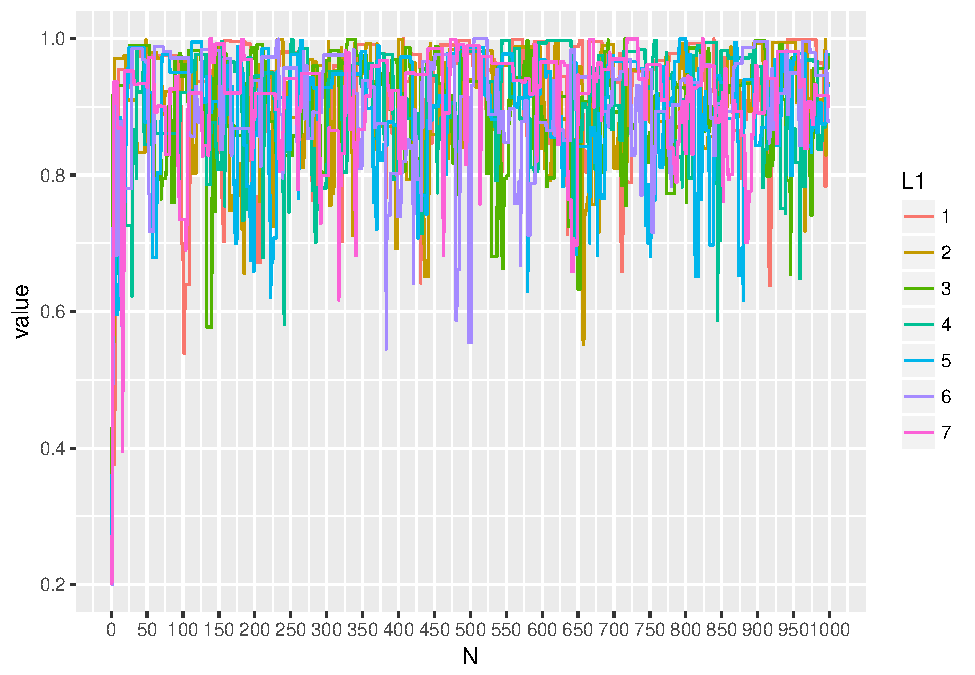
\includegraphics{Atlas-PS_6_files/figure-latex/unnamed-chunk-14-1.pdf}

It seems like the results from the first 50 observations are not too
great either, as approximately the first 25 observations are heavily
influenced by the starting value.

The takeaway here is that even though the \(\sqrt{R}\) seems good, it's
worth further inspection. The tools laid out in the chapter, graphical
and quantitative, can't effectively be used in isolation.


\end{document}
